%=========================================================================
% (c) 2011, 2012 Josef Lusticky <xlusti00@stud.fit.vutbr.cz>

\chapter{Contiki OS}
Only 2\% of all microprocessors that are sold today are used in PCs and the remaining 98\%
of all microprocessors are used in embedded systems~\cite{thesis-programming}.
The microprocessors
used in embedded systems have much smaller amounts of memory than PC computers.
The memory constraints make programming for embedded systems a challange.

Operating system Contiki is targeted at embedded systems supporting MSP430, AVR, ARM, x86
architecture and many others~\cite{contiki-docs}.
Contiki aims for maximum portability and therefore is written in C.
It is a feature-rich operating system and it
is possible to describe only some of its features in this thesis.

Contiki OS features lightweight stackless threads called Protothreads.
Protothreads are a new concept brought by Contiki to the embedded world,
they are extremely lightweight and compatible with standard C~\cite{paper-protothreads}.
Each Protothread does not require a separate stack which makes them perfectly
fit for usage in programming memory constrained embedded systems.
Protothreads are more detailed discussed in section~\ref{sec:contiki-protothreads}.

Contiki also features TCP/IP communication stack called uIP~(micro~IP)
that comforms to Request For Comments memorandums published by the Internet Engineering Task Force.
The uIP provides communication abilities using both IPv4 and IPv6~\cite{contiki-docs}.
Contiki with its uIP stack is IPv6 Ready Phase 1 certified
and therefore has the right to use the IPv6~Ready silver logo~\cite{ipv6ready-db}.
Before Contiki's uIP the embedded world considered IP to be too heavyweight.
That means all sooner available IP implementation for general purpose computers
were much bigger than the memory constrained embedded systems could use~\cite{interconnecting}.
The communication stack uIP is closely described in section~\ref{sec:contiki-uip}.

Next to the uIP Contiki is equipped with other communication stack called Rime.
Rime is a layered communication stack for sensor networks,
with much tinner layers than traditional architectures~\cite{paper-rime}.
Rime is designed to simplify the implementation of communication
protocols on low-power radios.
Rime is shortly discussed in section~\ref{sec:contiki-rime}.

Operating system Contiki, uIP and Protothreads are used by hundreds of companies in embedded devices in
such diverse systems as car engines, oil boring equipment, satellites, and container security systems~\cite{thesis-programming}.
The software is also used both in academic research
projects and in university project courses on embedded systems throughout the
world.

Contiki is developed by a group of developers from industry and academia
lead by Adam Dunkels from the Swedish Institute of Computer Science.
The Contiki team currently consists of sixteen developers from SICS,
SAP AG, Cisco, Atmel, NewAE and TU Munich~\cite{contiki-docs}.
Contiki is also deployed at RheinMain University in Wiesbaden.
The 3-clause BSD license is placing minimal restrictions on how Contiki can be redistributed.
Contiki version 1.0 was released in 2002, version 2.0 in 2007 and the latest version
at the time of writing was 2.5 released in 2011.
The actual development happens in a repository online using the Git version control system
accessible on Contiki homepage at \url{http://www.contiki-os.org/}.


%=========================================================================
% (c) 2011, 2012 Josef Lusticky <xlusti00@stud.fit.vutbr.cz>

\section{Protothreads}\label{sec:contiki-protothreads}
Protothreads provide a way to run C functions quasi-paralelly, that is, a C functions work in a way similiar to thread.
In Contiki Protothreads allow process to wait for incoming events. While waiting for an event to occur another function
can be run. The core of this solution is C switch statement used in conjuction with variable (called local continuation)
containing the position where the function was interrupted. Next time function continues from this point.

The advantage of Protothreads over ordinary threads is that a Protothread does not require a separate stack.
In memory constrained systems, the overhead of allocating multiple stacks can consume large amounts of
the available memory. In contrast, each Protothread only requires few bytes for storing the state of execution.

A Protothread is driven by repeated calls to the function in which the Protothread is running.
Each time the
function is called, the Protothread will run until it blocks or exits.
Protothreads are implemented using local continuations. A local continuation represents the current state
of execution at a particular place in the program, but does not provide any call history or local variables.

The Protothreads API consists of four basic operations: initialization (PT\_INIT()), execution (PT\_BEGIN()),
conditional blocking (PT\_WAIT\_UNTIL()) and exit (PT\_END()). On top of these, two convenience functions
are built: reversed condition blocking (PT\_WAIT\_WHILE()) and Protothread blocking (PT\_WAIT\_THREAD())~\cite{paper-protothreads}.

To understand how are Protothreads implemented and how do the actually work please refer
to appendix~\ref{app:protothreads} in which an example of usage is shown.

Since Protothreads are implemented using standard C, library providing Protothreads can be used everywhere C toolchain is available.
But there are some cons to consider. Because protothreads are stackless, a Protothread can only run within a single C function.
There is also no way of storing automatic local variables. And since Protothreads are implemented using C {\it switch} statement, and these can
not be nested, the code that uses Protothreads cannot use {\it switch} statements itself.
Workaround for storing local variables is to prepend them with the {\it static} keyword, which make them being put into data segment
by compiler and thus remembering the value between the function calls.


%=========================================================================
% (c) 2011, 2012 Josef Lusticky

\section{uIP}\label{sec:contiki-uip}
The TCP/IP protocol suite is often used for communication over the Internet as well as local networks.
uIP (micro IP) is a complete TCP/IP communication stack developed by Adam Dunkels
for memory constrained systems such as embedded systems.

Before uIP, the TCP/IP architecture was considered to be heavyweight
due to its perceived need for processing power and memory.
The IP protocol was seen as too large to fit into the constrained environment -
existing implementations of the IP protocol family for general purpose computers would need hundreds
of kilobytes, whereas a typical constrained system has only a few tens of kilobytes of memory~\cite{interconnecting}.
For this reason, several non-IP stacks were developed.

In the early 2000's, however, this view was challenged by lightweight implementations of the IP
protocol family for smart objects such as the uIP stack~\cite{interconnecting}.
uIP showed that the IP architecture would fit nicely into the typical constrained systems,
without removing any of the essential mechanisms from IP.
Note that these resources, which are considered constrained today, are fairly close to the
resources of general purpose computers that were available when IP was designed~\cite{interconnecting}.
Since its initial release, the uIP stack has become widely used in networked
embedded systems~\cite{interconnecting, thesis-programming}.

uIP provides two different application programming interfaces to programmers:
a BSD sockets-like API called Protosockets and raw event-driven API.
Protosockets are based on Protothreads putting the same limitation on them - such as
no way of storing automatic local variables and an impossibility of using the C {\it switch} statement.
Protosockets only work with TCP connections~\cite{contiki-docs}.
Since NTP uses UDP, Protosockets will not be further
discussed in this thesis. For more information about Protosockets
please refer to the Contiki documentation~\cite{contiki-docs}.

uIP contains only the absolute minimum of required features to fulfill the protocol standard.
It can only handle a single network interface and contains the IP, ICMP, UDP and TCP protocols~\cite{contiki-docs}.
In order to reduce memory requirements and code size,
the uIP implementation uses an event-based API, which is fundamentally different
from the most common TCP/IP API, the BSD sockets API, present on Unix-like systems
and defined by the POSIX standard~\cite{thesis-programming,posix}.
An application is invoked in response to certain events and
it is up to the application that is receiving events from uIP to handle all
work with data to be transmitted. E.g. if the data is lost in the network,
the application will be invoked and then has to resend the data.
This approach is based on the fact that it should be simple for the application
to rebuild the same data.
This way, the uIP stack does not need to use explicit dynamic memory allocation.
Instead, it uses a single global buffer for holding packets and has a fixed
table for holding the connection state.
The global packet buffer is large enough to contain one packet of maximum size~\cite{contiki-docs}.

When a packet arrives from the network, the device driver places it in the
global buffer and calls the TCP/IP stack.
If the packet contains data, the TCP/IP stack will notify the corresponding application.
Because the data in the buffer will be overwritten by the next incoming packet,
the application will either have to act immediately on the data or copy the data into
its own buffer for later processing.
The packet buffer will not be overwritten by new packets before the application has processed the data~\cite{contiki-docs}.
Packets that arrive when the application is processing the data must be queued,
either by the network device or by the device driver.
That means uIP relies on the hardware when it comes to buffering.
Most single-chip Ethernet controllers have on-chip buffers
that are large enough to contain at least 4 maximum sized Ethernet frames~\cite{contiki-docs}.
This way, uIP does not have to have its own buffer structures and thus
only a minimal memory amount is required.
Possible packet loss is a trade-off for minimalism and ability to communicate using TCP/IP.
It is not such a big deal for communication using TCP on the transport layer
because of the acknowledgement scheme used in TCP to prevent data loss.
However data carried on UDP can be irrecoverably lost.

As was expected, measurements show that the uIP implementation provides very low
throughput, particularly when communicating with a PC host~\cite{thesis-towards}.
However, small systems that uIP is targeting, usually do not produce enough data
to make the performance degradation a serious problem~\cite{thesis-towards}.

Despite being so small, uIP is not only RFC compliant, but also IPv6 Ready Phase 1 certified.
uIP is written in the C programming language and it is fully integrated with the Contiki operating system.
In uIP, there are even some more tricks to shrink the stack
but complete uIP description is outside the scope of this thesis.
Please refer to the Contiki documentation for more details~\cite{contiki-docs}.


%=========================================================================
% (c) 2011, 2012 Josef Lusticky <xlusti00@stud.fit.vutbr.cz>

\section{Rime}\label{sec:contiki-rime}
Typical sensor devices are equipped with 8-bit microcontrollers,
code memory on the order of 100 kilobytes, and less than
20 kilobytes of RAM~\cite{paper-contiki}.
Moore's law predicts that these devices
can be made significantly smaller and less expensive
in the future. While this means that sensor networks can
be deployed to greater extents, it does not necessarily imply
that the resources will be less constrained~\cite{paper-contiki}.

The purpose of Rime is to simplify implementation of
sensor network protocols and facilitate code reuse~\cite{paper-rime}. 
The communication primitives in the Rime stack were choosen
based on what typical sensor network protocols use~\cite{contiki-docs}.
Rime can significantly simplify protocol implementation
with only a small increase in resource requirements.
The code footprint of Rime is less than two kilobytes and the
data memory requirements on the order of tens of bytes~\cite{paper-rime}.
To reduce memory footprint Rime uses a single buffer for
both incoming and outgoing packets similar to uIP. Layers
that need to queue data copy the data to dynamically
allocated queue buffers~\cite{paper-rime}.

Rime is undoubtely an interesting communication stack, but
as NTP is designed to run on top of IP, Rime will not be discussed
in this thesis further.
Please consult the Contiki documentation~\cite{contiki-docs} if you desire
more details about Rime.


%=========================================================================
% (c) 2011, 2012 Josef Lusticky

\section{Kernel and processes}\label{sec:contiki-kernel}
The kernel in Contiki is event-driven providing cooperative multitasking
environment, but the system supports preemptive
multithreading that can be applied on a per-process basis~\cite{video}.
The preemption is not implemented in the kernel, but
preemptive multithreading is implemented as a library that is linked only with programs that
explicitly require multithreading~\cite{paper-contiki}.
The kernel itself contains no platform specific code, it implements only CPU multiplexing and
lets device drivers and applications communicate directly with hardware~\cite{video}.

From high level of abstraction,
applications in Contiki OS are implemented and run as processes.
Protothreads, the lightweight threads described in section~\ref{sec:contiki-protothreads},
are used in Contiki to implement processes.
Both the Contiki kernel and Contiki applications use
Protothreads extensively to achieve cooperative multitasking~\cite{contiki-wiki-faq}.
Every Contiki process consists of a process control block and a process thread~\cite{contiki-wiki-processes}.
The process control block contains run-time information about the process and
the process thread contains the code of the process.
Among other things, the process control block contains
textual name of the process, pointer to the process thread and state of the process.
The process thread is implemented as a single Protothread,
that is invoked from the process scheduler in the Contiki kernel~\cite{contiki-wiki-processes}.

From low level of abstraction,
every application is implemented as a simple C function
and the process control block remembers the actual state of execution of this function
in the same way as the local continuation works by Protothreads.
Processes are therefore running quasi-parallely in Contiki.

\bigskip
\begin{lstlisting}[caption=Process control block in Contiki OS]
struct process {
	struct process *next;
	const char *name;
	int (* thread)(struct pt *, process_event_t, process_data_t);
	struct pt pt;
	unsigned char state, needspoll;
	};
\end{lstlisting}

Process control block is not declared or defined directly,
but through the {\it{PROCESS()}} macro.
This macro takes two parameters: the variable name of the process control block
and a textual name of the process,
which is used in debugging and when printing out lists of active processes to users~\cite{contiki-wiki-processes}.

All code execution is initiated by the Contiki kernel
that acts like a simple dispatcher calling these functions~\cite{contiki-docs}.
Just like Protothreads, processes are also implemented using macros,
making them fully standard C compatible.

In Contiki, code run in either of two execution contexts:
cooperative, in which code never preempts other code, and preemptive,
which preempts the execution of cooperative code and returns control
when preemptive code is finished.
Processes always run in cooperative mode,
whereas interrupt service routines and real-time timers run in preemptive mode~\cite{contiki-wiki-processes}.
Code running in both execution contexts illustrates figure~\ref{fig:contiki-execution-context}.

\begin{figure}
  \centering
  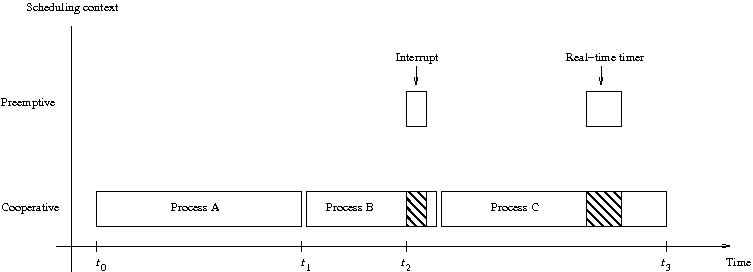
\includegraphics[width=13cm,keepaspectratio]{fig/Execution-contexts.png}
  \caption{Contiki execution contexts by A. Dunkels}
  \label{fig:contiki-execution-context}
\end{figure}

Interprocess communication is done by posting events in Contiki OS -
processes communicate with each other by posting events to each other~\cite{paper-contiki}.
There are two types of events: synchronous and asynchronous.
Synchronous events are directly delivered to the receiving process when posted and
can only be posted to a specific processes~\cite{contiki-wiki-processes}.
Because synchronous events are delivered immediately,
posting synchronous event is equivalent to a function call:
the process to which an event is delivered is directly invoked,
and the process that posted the event is blocked
until the receiving process has finished processing the event~\cite{contiki-wiki-processes}.

Asynchronous events are delivered to the receiving process
some time after they have been posted~\cite{contiki-wiki-processes}.
Before delivery, the asynchronous events are held on event queue inside Contiki kernel.
The kernel loops through this event queue and delivers
the event to the process by invoking the process. 
The receiver of an asynchronous event can be either a specific process
or all running processes~\cite{contiki-wiki-processes}.

%! paper-contiki - dunkels04contiki
%Being able to power down the device
%when the network is inactive is often required way to reduce energy consumption.
%Power conservation mechanisms
%depend on both the applications and the network protocols.
%The Contiki kernel contains no explicit power
%save abstractions, but lets the the application specific parts
%of the system implement such mechanisms.
%To help the application decide when to power down the system, the event
%scheduler exposes the size of the event queue.
%This information can be used to power down the processor when there
%are no events scheduled.
%! paper-contiki

%As stated before, Contiki is well documented and you can find out more about
%the kernel as well as the system in the documentation~\cite{contiki-docs}.


%=========================================================================
% (c) 2011, 2012 Josef Lusticky

\section{Timers}\label{sec:contiki-timers}
The Contiki kernel does not provide support for timed events,
instead an application that wants to use timers needs to explicitly use a timer library.
The timer library provides functions for setting, resetting and restarting timers,
and for checking if a timer has expired.
An application must manually check if its timers have expired - this is not done automatically~\cite{contiki-docs}.

Contiki has one clock library and a set of timer libraries: timer, stimer, ctimer, etimer, and rtimer~\cite{contiki-wiki-timers}.
The clock library provides functionality to handle the system time and to block the CPU for short time periods.
It is the interface between Contiki and the platform-specific hardware clock~\cite{contiki-docs}.
The timer libraries are implemented with the functionality of the clock library as a base~\cite{contiki-wiki-timers}.

The timer and stimer libraries provide the simplest form of timers and are used to check whether a time period has passed.
The difference between these two is the resolution of time -
timers use system clock ticks, whose value is incremented when an interrupt from the hardware clock occurs,
while stimers use seconds to offer much longer time periods~\cite{contiki-wiki-timers}.
The value representing seconds is also incremented in the interrupt service routine (ISR),
but only when enough clock ticks since last increment occurred.
The number of clock ticks within one second is represented by the
{\it{CLOCK\_SECOND}} macro provided by the clock library.
That means there are {\it{CLOCK\_SECOND}} interrupts from the hardware clock per second.
The usage of the timer library and {\it{CLOCK\_SECOND}} macro is shown in appendix~\ref{app:protothreads}.

The simplest timer and stimer libraries are not able to post an event when a timer expires.
Event timers should be used for this purpose.
Event timers (etimer library) provide a way to generate timed events.
An event timer will post an event to the process that set the timer when the
event timer expires~\cite{contiki-docs}.
The etimer library is implemented as a Contiki process and uses the timer library as a base.

Callback timers (ctimer library) provide a timer mechanism that calls a specified
C function when a ctimer expires~\cite{contiki-docs}.
Thus, they are especially useful in any code that does not have an
explicit Contiki process~\cite{contiki-wiki-timers}.

The Real-time timers (rtimer library) handle the scheduling and execution of
real-time tasks with predictable execution times~\cite{contiki-docs}.
The rtimer library provides real-time task support through callback functions -
the rtimer immediately preempts any running Contiki process in order to let the real-time tasks
execute at the scheduled time~\cite{contiki-wiki-timers}.
This behaviour is illustrated in figure~\ref{fig:contiki-execution-context}.
The rtimer library uses a separate hardware clock
to allow a higher clock resolution~\cite{contiki-wiki-timers}.
The small part of the rtimer library is architecture-agnostic,
but the particular implementation is platform-specific.

